\chapter{Two-dimensional compressive sensing (2DCS)}
\label{chap:2dcs}

\section{Methodology}
\label{sec:2dmetho}
The compressive sensing (CS) of two-dimensional, spatial signals is the more intuitive of its applications as it is easier to visualize. As we will see later on, the CS of image signals can be simplified either by flattening it to one dimension or by patches. The general workflow that arises from image CS is as follows:

\begin{enumerate}
	\item Define the compression ratio $m/n$, where $n$ is the signal size, and $m$ is the desired size of the compressed signal.
	\item Draw $m$ random indices from the signal without replacement and store this as a vector $\xi$.
	\item Extract the row vectors of the desired $n \times n$ sparsifying basis $\bm\Psi$ corresponding to the indices in $\xi$, and stack these to form the sensing matrix $\bm\Phi$.
	\item With the desired reconstruction algorithm, perform the minimization \eqref{eq:min-l1} to obtain the reconstructed signal $\bm\hat{\vec{x}}$.
\end{enumerate}

In the case of high-definition images, it is usually more practical and yields better results if the image is first divided into smaller, manageable patches and apply the above steps per patch, then stitch the patches back together at the end to form the final reconstructed image.


\section{Test case: Sinusoidal pattern}
\label{sec:2dsin}
Image signals are commonly expressed sparsely as a linear superposition of a finite number of 2D sinusoidal patterns. In Fig. \ref{fig:2dsin}, $64 \times 64$ pixel sinusoidal patterns were generated, corresponding to $\sin(x)$ (sine wave traveling horizontally), $\sin(y)$ (sine wave traveling vertically), $\sin(x+y)$ (sine wave traveling diagonally), and $\sin(x) + \sin(y)$ (egg tray pattern). In each case, all frequency components are 4 Hz. Figure \ref{fig:2dsin-masked} visualizes the compressed image when a random sample of 5\% is taken from the signal. The actual compressed signal that is seen by the reconstruction algorithm is a one-dimensional vector containing the sampling points. For reconstruction, the algorithm used is CVXPY, which casts the minimization problem \ref{eq:min-l1} as a convex optimization problem, and directly minimizes the $\ell_1$ norm \cite{cvxpy,cvxpy_rewriting}. From the 5\% of samples taken from the original image, the reconstructed signals are shown in Fig. \ref{fig:2dsin-recovered}, each of which has a mean-squared error (MSE) of no more than 0.06. Exact reconstruction is attained for the pure horizontal and pure vertical sine waves, as well as the egg tray pattern. Additional artifacts are present in the reconstructed diagonal sine wave, particularly at the boundaries.

\begin{figure}[tb]
	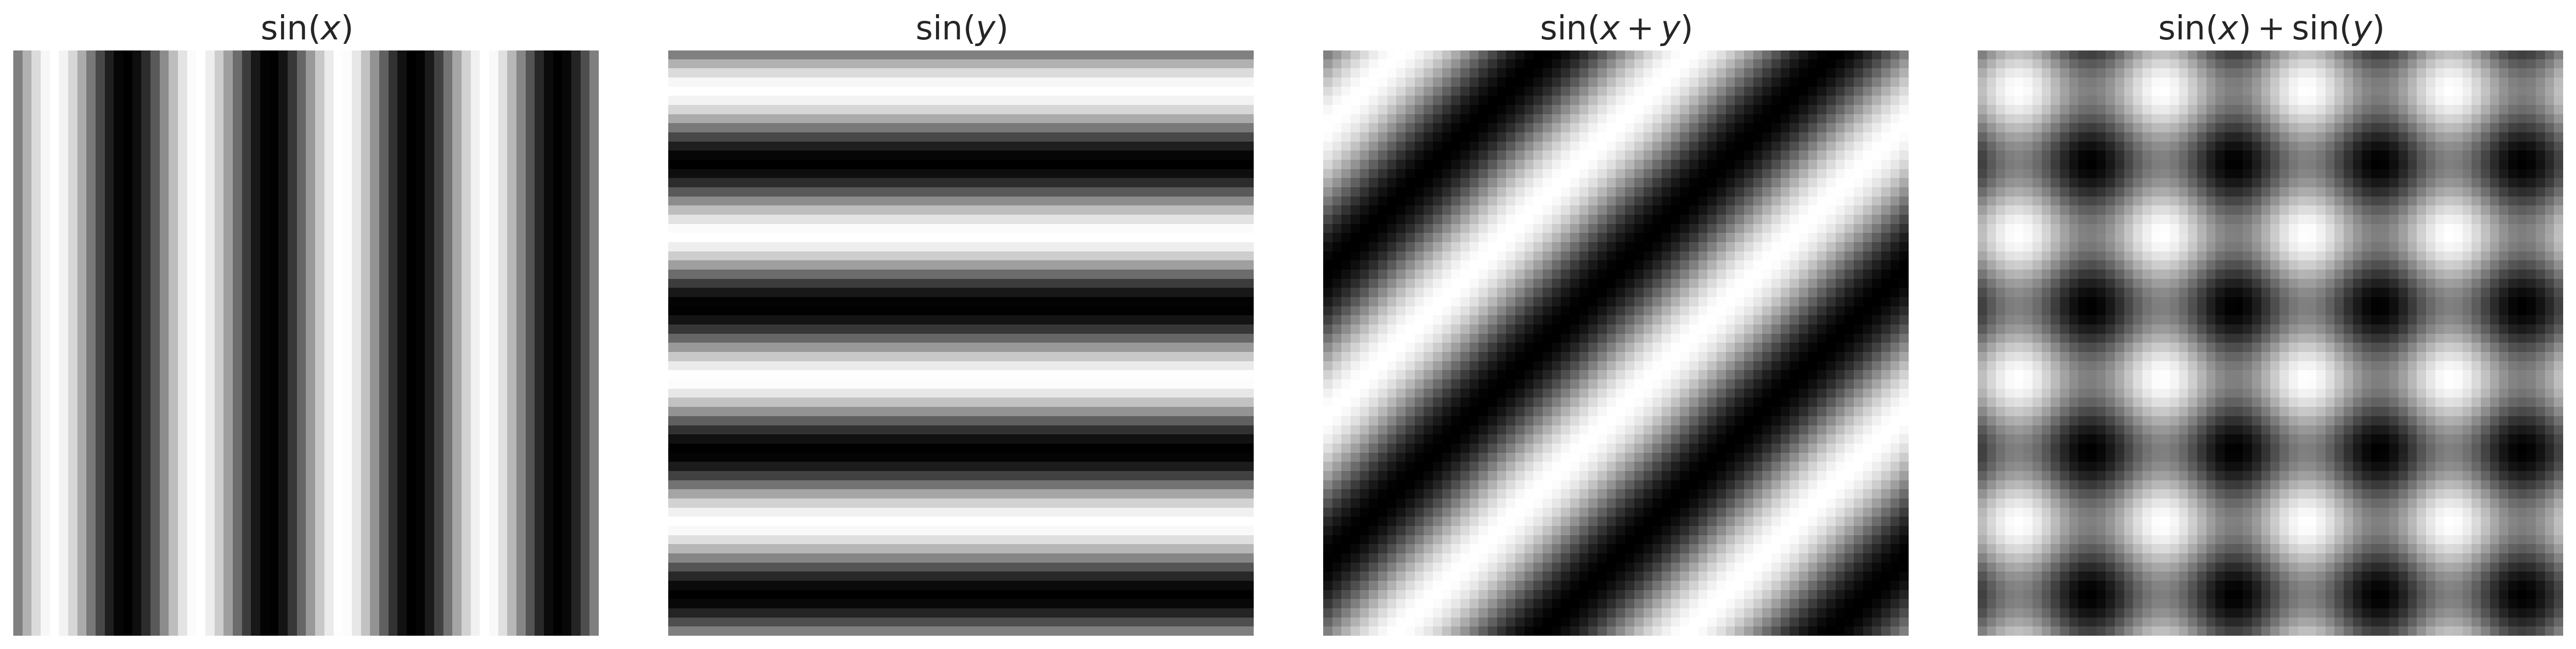
\includegraphics[width=\textwidth]{2dsin.png}
	\caption{Test 2D sinusoid patterns.}
	\label{fig:2dsin}
\end{figure}

\begin{figure}[tb]
	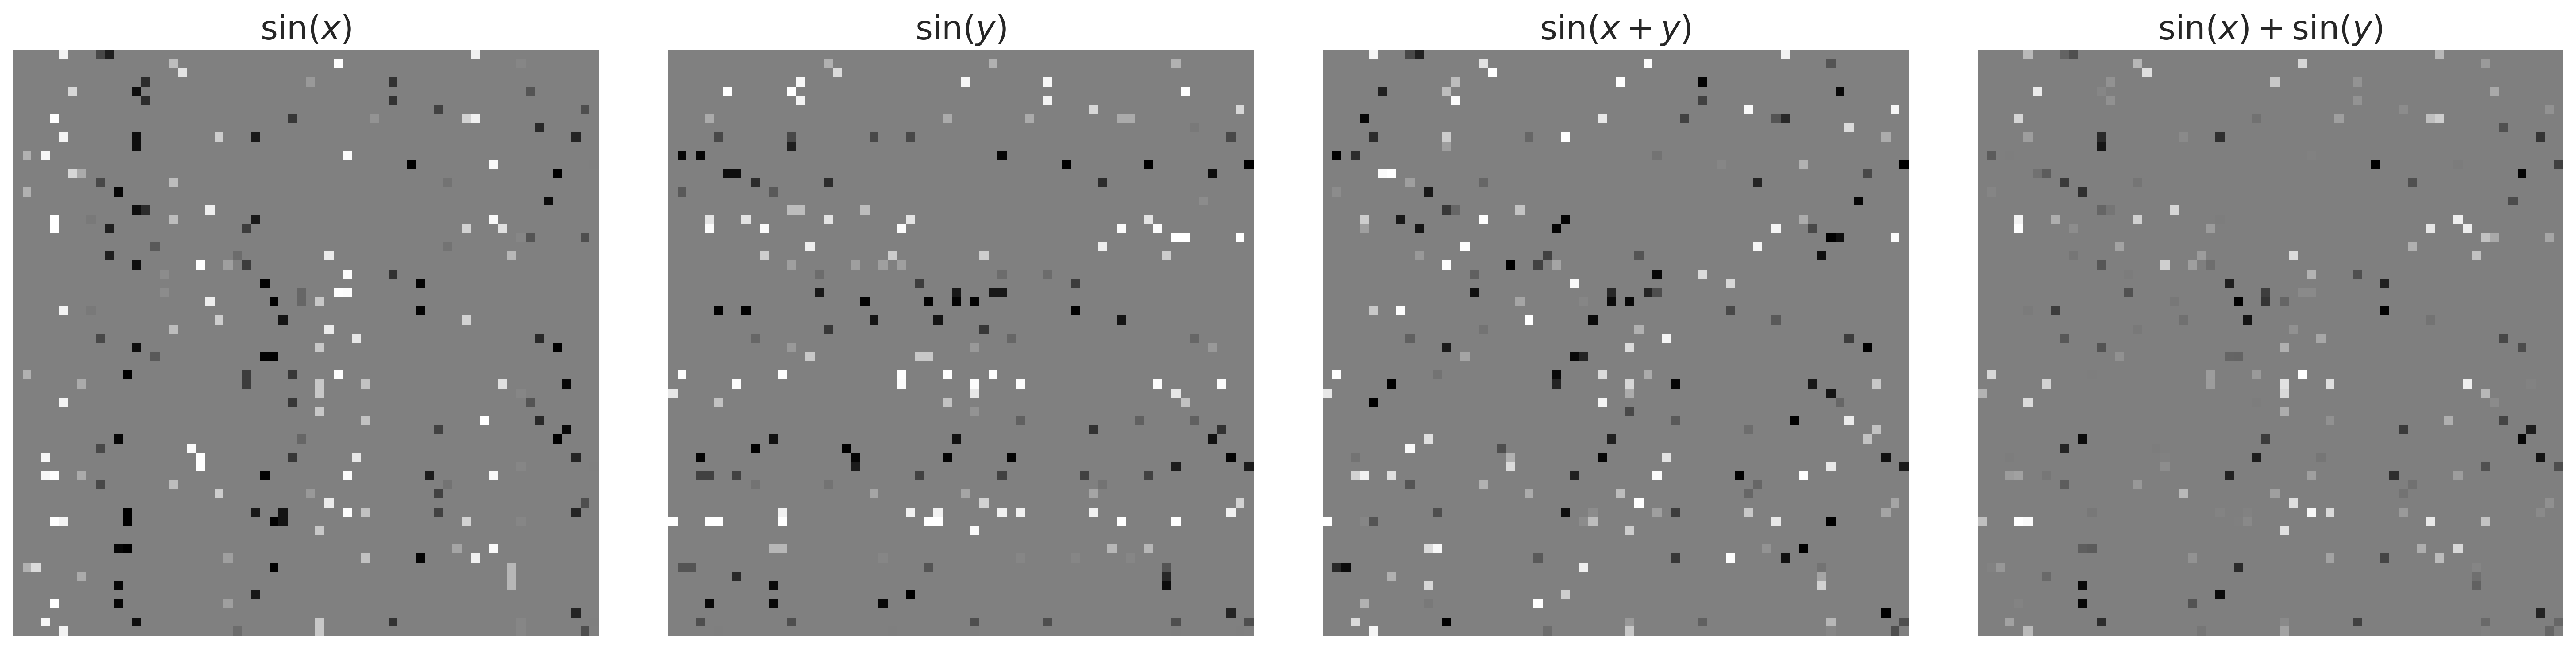
\includegraphics[width=\textwidth]{2dsin-masked.png}
	\caption{Visualization of compressed sinusoid patterns.}
	\label{fig:2dsin-masked}
\end{figure}

\begin{figure}[tb]
	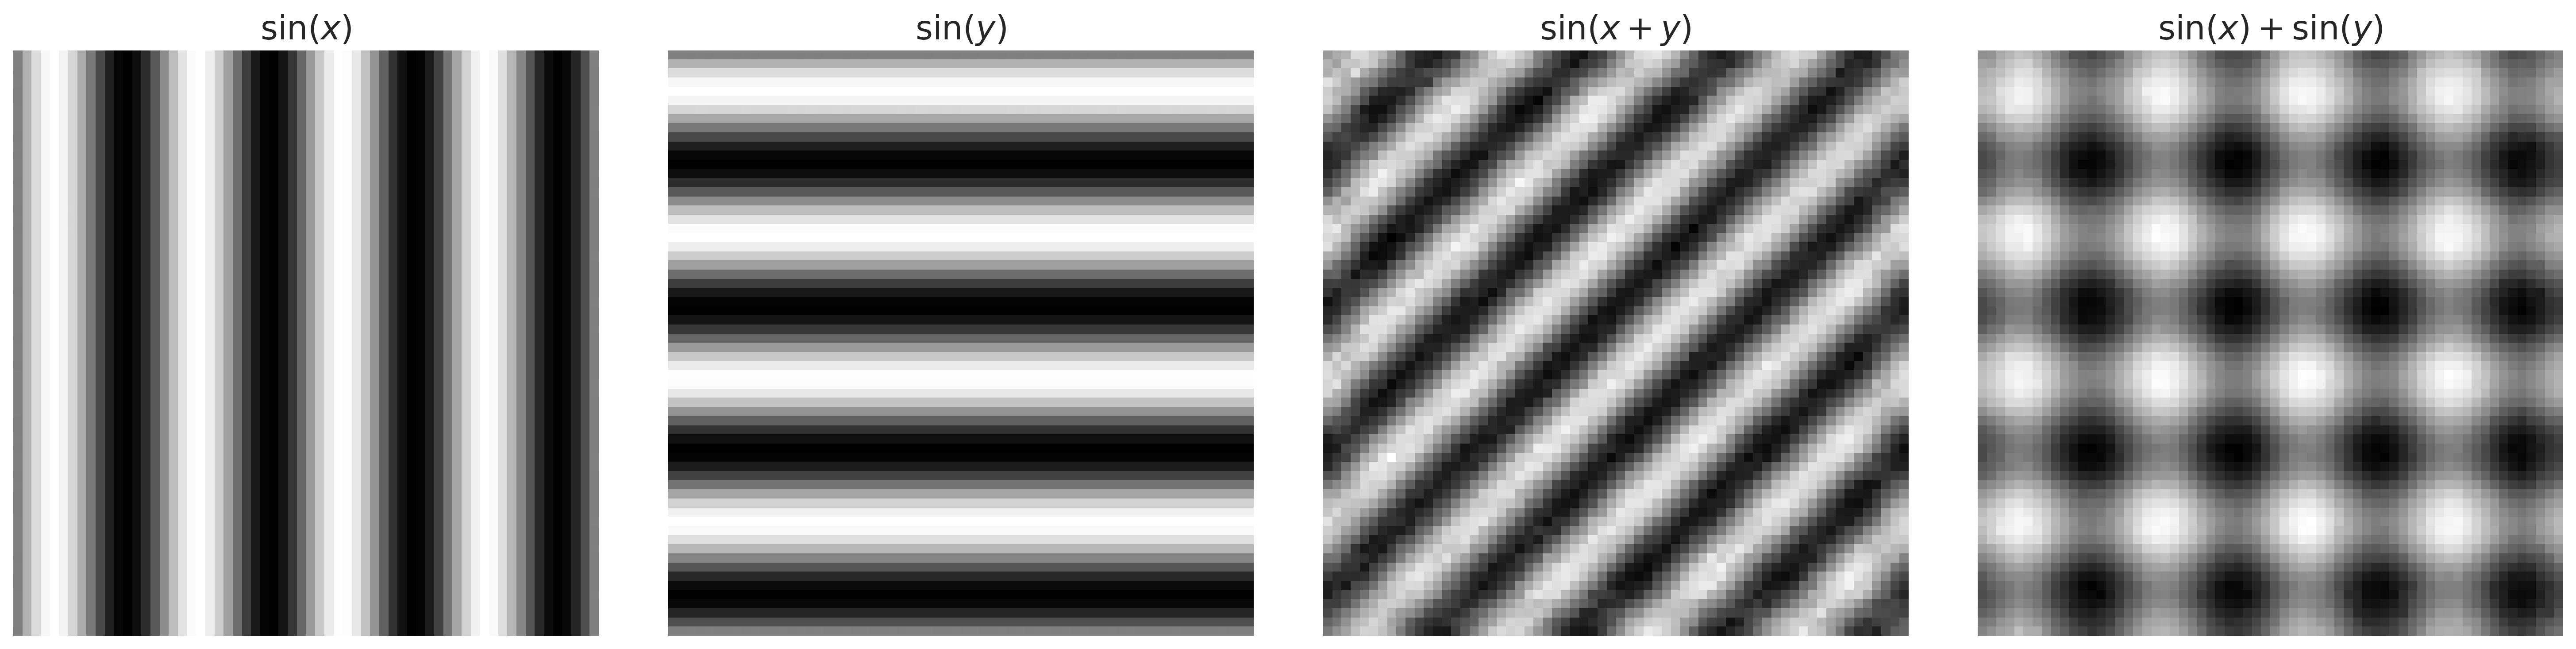
\includegraphics[width=\textwidth]{2dsin-recovered.png}
	\caption{Reconstructed sinusoid patterns from 5\% of samples from original image.}
	\label{fig:2dsin-recovered}
\end{figure}


\section{Image with multiple sinusoids}
\label{sec:2dmultisin}
For this section, the image used is M.C. Escher's \textit{Relativity}, an example of a more complex image consisting of various sinusoidal patterns. The original image has dimensions of $1600 \times 981$ pixels, for a total of 1,569,600 pixels. This would require the construction of a 1,569,600 $\times$ 1,569,600 sparsifying matrix, or $\approx 2 \times 10^{12}$ entries. Assuming that the matrix would be stored as 32-bit floating point numbers, this process alone would take up $\approx 8$ GB of RAM, and it would be highly impractical to process similar images as a whole. A workaround is to split it into smaller, manageable patches. For this image in particular, it was first resized to $1600 \times 976$ pixels so that it could be equally divided into a grid of $16 \times 16$, each with a dimension of $100 \times 61$ pixels. After compressively sensing each patch and stitching all patches at the end, the reconstructed image is shown in Fig. \ref{fig:relativity-recovered}. Selected patches are shown side-by-side with their reconstructed counterparts in Fig. \ref{fig:relativity-dominant-slices}, corresponding to patches dominated by horizontal sinusoids, vertical sinusoids, diagonal sinusoids, and patches with no dominant pattern.


\begin{figure}[tb]
	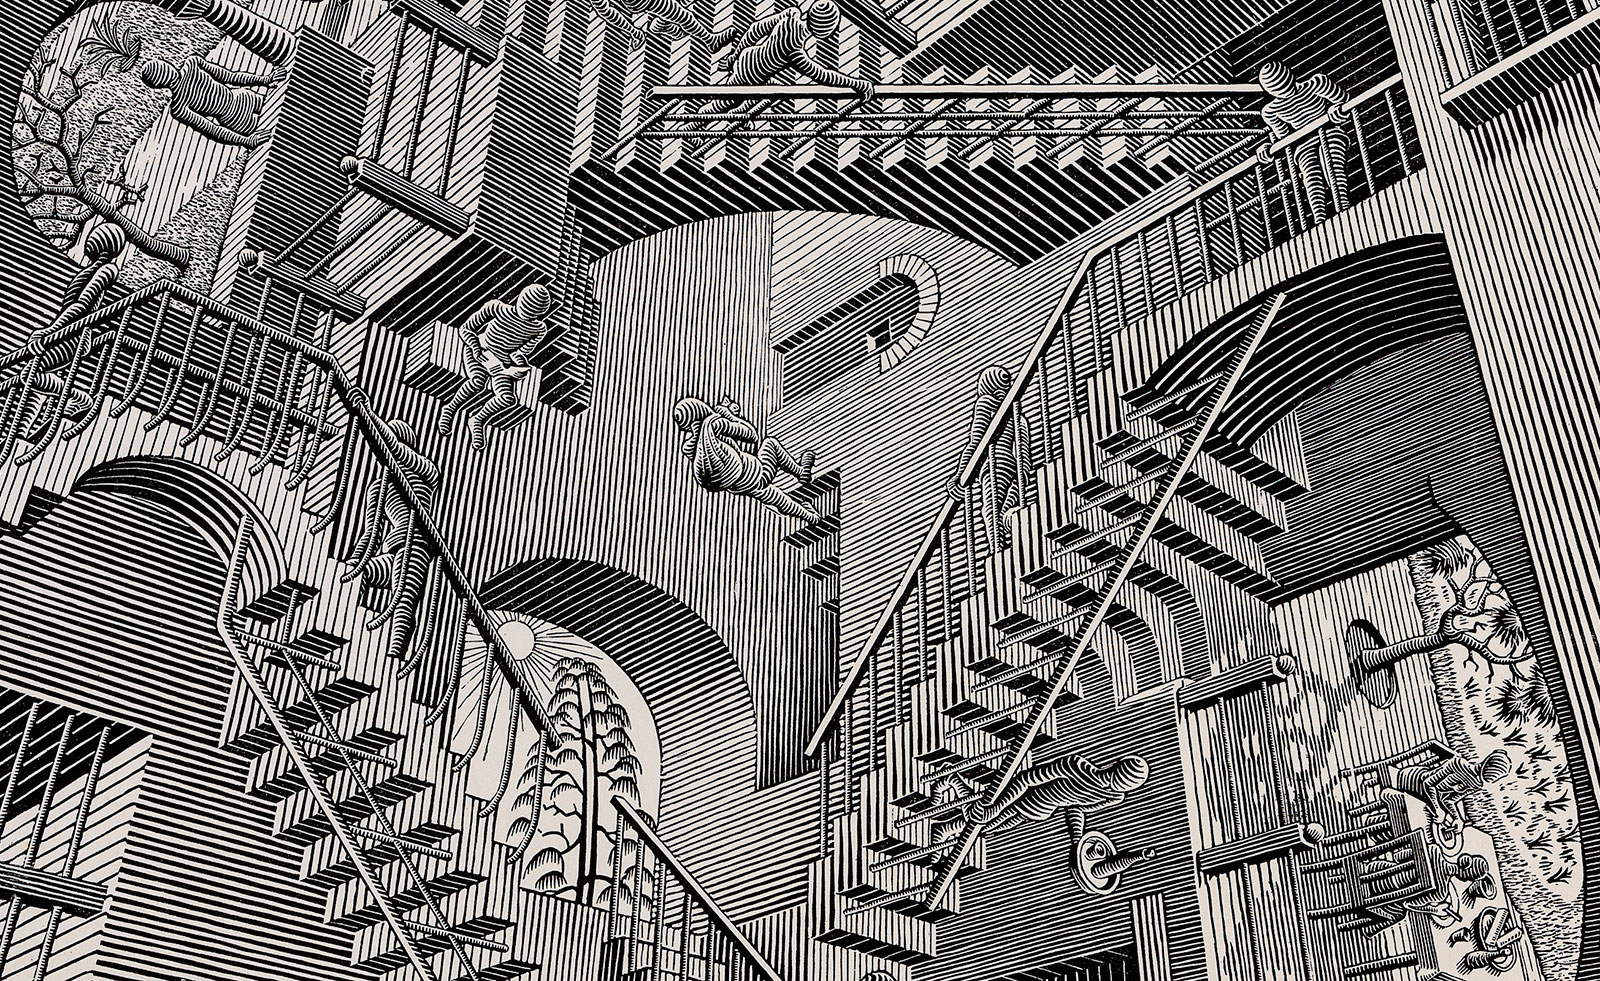
\includegraphics[width=\textwidth]{relativity.jpg}
	\caption{\textit{Relativity} by M.C. Escher, a complex image consisting of various sinusoidal patterns.}
	\label{fig:relativity}
\end{figure}

\begin{figure}[tb]
	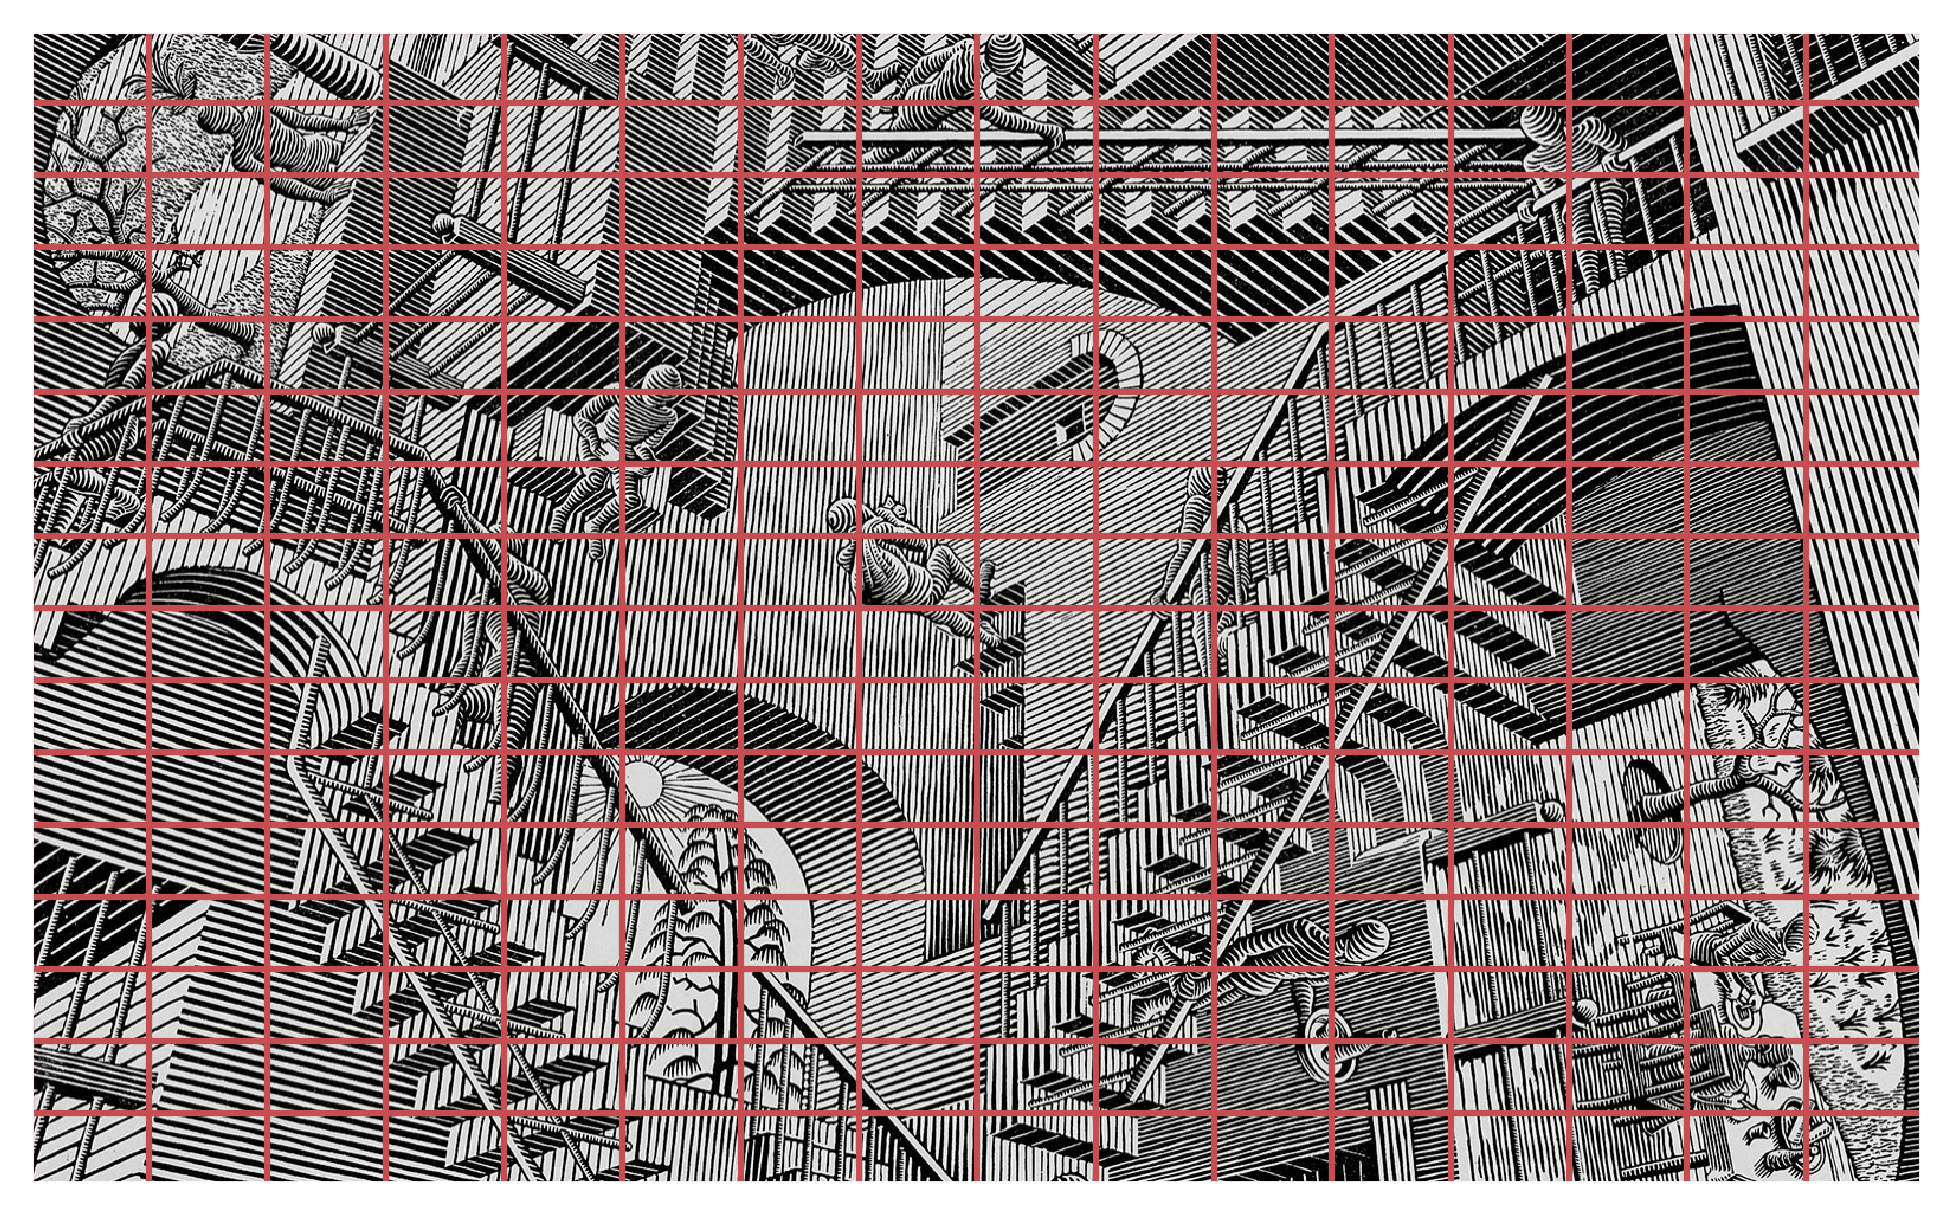
\includegraphics[width=\textwidth]{relativity-slices.png}
	\caption{Test image divided into a grid of $16 \times 16$.}
	\label{fig:relativity-slices}
\end{figure}


\section{Simultaneous compression \& encryption}
Because of the way compressively sensed images are coded with the sensing matrix, the use of CS as an encryption algorithm arises naturally. Consider the logistic map

\begin{equation}\label{eq:logistic-map}
	x_{n+1} = r x_n \qty(1 - x_n)
\end{equation}

\noindent which is often used as an archetypal example of deterministic chaotic behavior when $r \in [3.57, 4]$. Within these values, the sequences produced by varying the initial value $x_0$ rapidly diverge from each other. Thus, this can become an encryption system by treating the parameters $r$ and $x_0$ as the encryption keys, and \eqref{eq:logistic-map} as the hash function. 